\documentclass[12pt,letterpaper]{article}
\usepackage[papersize={8.5in,11in}]{geometry}
\usepackage{fullpage}
\usepackage{gensymb}
\usepackage[utf8]{inputenc}
\usepackage{graphicx}
\usepackage{amsmath,amsfonts,mathtools,amsthm,subcaption}
\author{Jiaqi Zhu \\Amath 482, Winter 2020}
\title{Neutral Networks for Classifying Fashion MNIST}

\begin{document}
\maketitle
\begin{abstract}
This project aims to train a fully-connected and convolutional neural network model to build a classifer for the popular MNIST dataset which contains images of 10 different classes of fashion items. We will try several different neutral network architectures with different hyperparameters to try to construct a model with best performance and highest accuracy.  
\end{abstract}

\section*{I. Introduction and Overview}
Neural Network is either a biological neural network, made up of real biological neurons, or an artificial neural network, for solving artificial intelligence (AI) problems. These artificial networks may be used for predictive modeling and application where they can be trained via dataset. For this project, we were supposed to train a fully-connected neural network for part I and a convolutional neural network model for part II within a dataset of images of 10 different classes of fashion items. For both parts, we try different neural network achitectures with different hyperparameters to try to construct a model with highest accuracy and make a comparision between the two models we selected in the end. 

\section*{II. Theoretical Background}
\subsection*{Neural Network}
Neural networks are a set of algorithms. They interpret sensory data through a kind of machine perception, labeling or clustering raw input. The patterns they recognize are numerical, contained in vectors, into which all real-world data, be it images, sound, text or time series, must be translated.
\\Neural networds are composed of several layers (input or output layers). These input-weight products are summed and then the sum is passed through a node’s so-called activation function, to determine whether and to what extent that signal should progress further through the network to affect the ultimate outcome, say, an act of classification.
\subsection*{Fully-connected Neural Network}
For a given layer, every neuron is connected to every neuron in the previous layer.  We call those typesof layersfully-connectedordense.  When all of the layers are of that type, we say that it is a fully-connected network. The number of neurons in each layer is called the width of thelayer.  The number of layers is called the depth of the network. 
\subsection*{Convolutional Neural Network (CNN)}
A convolutional neural network consists of an input and an output layer, as well as multiple hidden layers. The hidden layers of a CNN typically consist of a series of convolutional layers that convolve with a multiplication or other dot product. The activation function is commonly a RELU layer, and is subsequently followed by additional convolutions such as pooling layers, fully connected layers and normalization layers, referred to as hidden layers because their inputs and outputs are masked by the activation function and final convolution.

\section*{III. Algorithm Implementation and Development}
\subsection*{Part I}
After following the homwork guidline to preprocess the data, I start to try to do experiment over different neural network architectures with different hyperparameters to get one best fully-connected Neural Networks model with highest accuracy. 
\\
\\For the first experiment, I start with a simple three-layer Neural Network with optimizer Adam. For the first layer, I flattened the data. The second layer is a fully conected layer with 250 neurons and ReLu activation function. The third layer is a fully conected layer with 10 neurons for classification and a softmax activation function. At the 20th epoch, the validation accuracy is $89.36\%$ and the training accuracy is $93.7\%$. 
\\
\\For the second experiment, we add two more hidden fully-connected layers, one with 100 neurons and one with 10 neurons. At the 20th epoch, the validation accuracy is $87.94\%$ and the training accuracy is $91.7\%$.
\\
\\For the third experiment, we just keep the simple three-layer Neural Network but with a different optimizer sgdm, stochastic gradient descent with momentum, At the 20th epoch, the validation accuracy is $86.7\%$ and the training accuracy is $89.28\%$.
\\
\\ For the fourth experiment, we just keep the simple three-layer Neural Network but with 100 neurons to test the influence of the width of the layers. At the 20th epoch, the validation accuracy is $86.46\%$ and the training accuracy is $86.8\%$.
\\
\\ For the fifth experiment, we also keep the simple fully-connected layers but with a different activation function At the 20th epoch, the validation accuracy is $88.72\%$ and the training accuracy is $93\%$.
\\
\\For the sixth experiment, we also keep the simple fully-connected layers but changing the hyperparamters learning rate and regularization parameter. When I changed the regularization parameter to 0.001, At the 20th epoch, the validation accuracy is $88.2\%$ and the training accuracy is $90.2\%$. We can see the difference between the validation and training accuracy become smaller which means that there's less overfitting problem; When I changed the learning rate to 0.0001, at the 20th epoch, the validation accuracy is $88.36\%$ and the training accuracy is $90\%$;
\\
\\From all of the experiments I did, I would choose the model of the first experiment.
\subsection*{Part II}
 Similar to the above procedure, we will adjust the the convolutional neural network stucture, the number of filters, filter sizes, strides padding options and pool sizes then come up with a best convolutional neural network model with highest accuracy. 
\\
\\For the first experiment, we have the structure starting with input $\rightarrow$ convolutional layer with 6 filters, 5 by 5 filter size and same padding with tanh activation function $\rightarrow$ average Pooling layer with pool size 2 and stride size 2$\rightarrow$convolutional layer with 16 filters, 5 by 5 filter size and no padding with tanh activation function $\rightarrow$ average Pooling layer with pool size 2 and stride size 2$\rightarrow$convolutional layer with 120 filters, 5 by 5 filter size and no padding with tanh activation function$\rightarrow$ fully connected layer with 84 output size with tanh activation $\rightarrow$ fully connected layer with 10 output size with softMax and Classification Layer. At the 5th epoch, the validation accuracy is $88.06\%$ and the training accuracy is $88.7\%$;
\\
\\For the second experiment, we keep the same structure but change the activation function back to reluLayer. At the 5th epoch, the validation accuracy is $88.14\%$ and the training accuracy is $89.62\%$;
\\
\\For the third experiment, we will change the average Pooling layer to Max Pooling layer with pool size 2 and stride size 1 as well as the number of filter and filter size. Then we have the structure starting with input $\rightarrow$ convolutional layer with 32 filters, 3 by 3 filter size and same padding withreluLaye activation function $\rightarrow$ max Pooling layer with pool size 2 and stride size 1$\rightarrow$convolutional layer with 64 filters, 3 by 3 filter size and no padding with reluLaye activation function $\rightarrow$ max Pooling layer with pool size 2 and stride size 1$\rightarrow$convolutional layer with 128 filters, 3 by 3 filter size and no padding with reluLayer activation function$\rightarrow$ fully connected layer with 256 output size with reluLaye activation $\rightarrow$ fully connected layer with 10 output size with softMax and Classification Layer. At the 5th epoch, the validation accuracyis $91.1\%$ and the training accuracy is $94\%$. 
\\
\\From all of the experiments I did, I would choose the model of the third experiment.
\section*{IV. Computational Results}

\subsection*{Part I}
As I mentioned before, I decided my final full connected neural network model to start with a simple three-layer Neural Network with optimizer Adam. For the first layer, I flattened the data. The second layer is a fully conected layer with 250 neurons and ReLu activation function. The third layer is a fully conected layer with 10 neurons for classification and a softmax activation function. At the 20th epoch, the validation accuracy is $89.66\%$ and the training accuracy is $93.7\%$.  For the testing data, the prediction accuracy is $88.2\%$ given by the following confusion matrix. 

\begin{figure}[ht]
\begin{subfigure}{.5\textwidth}
  \centering
  % include first image
  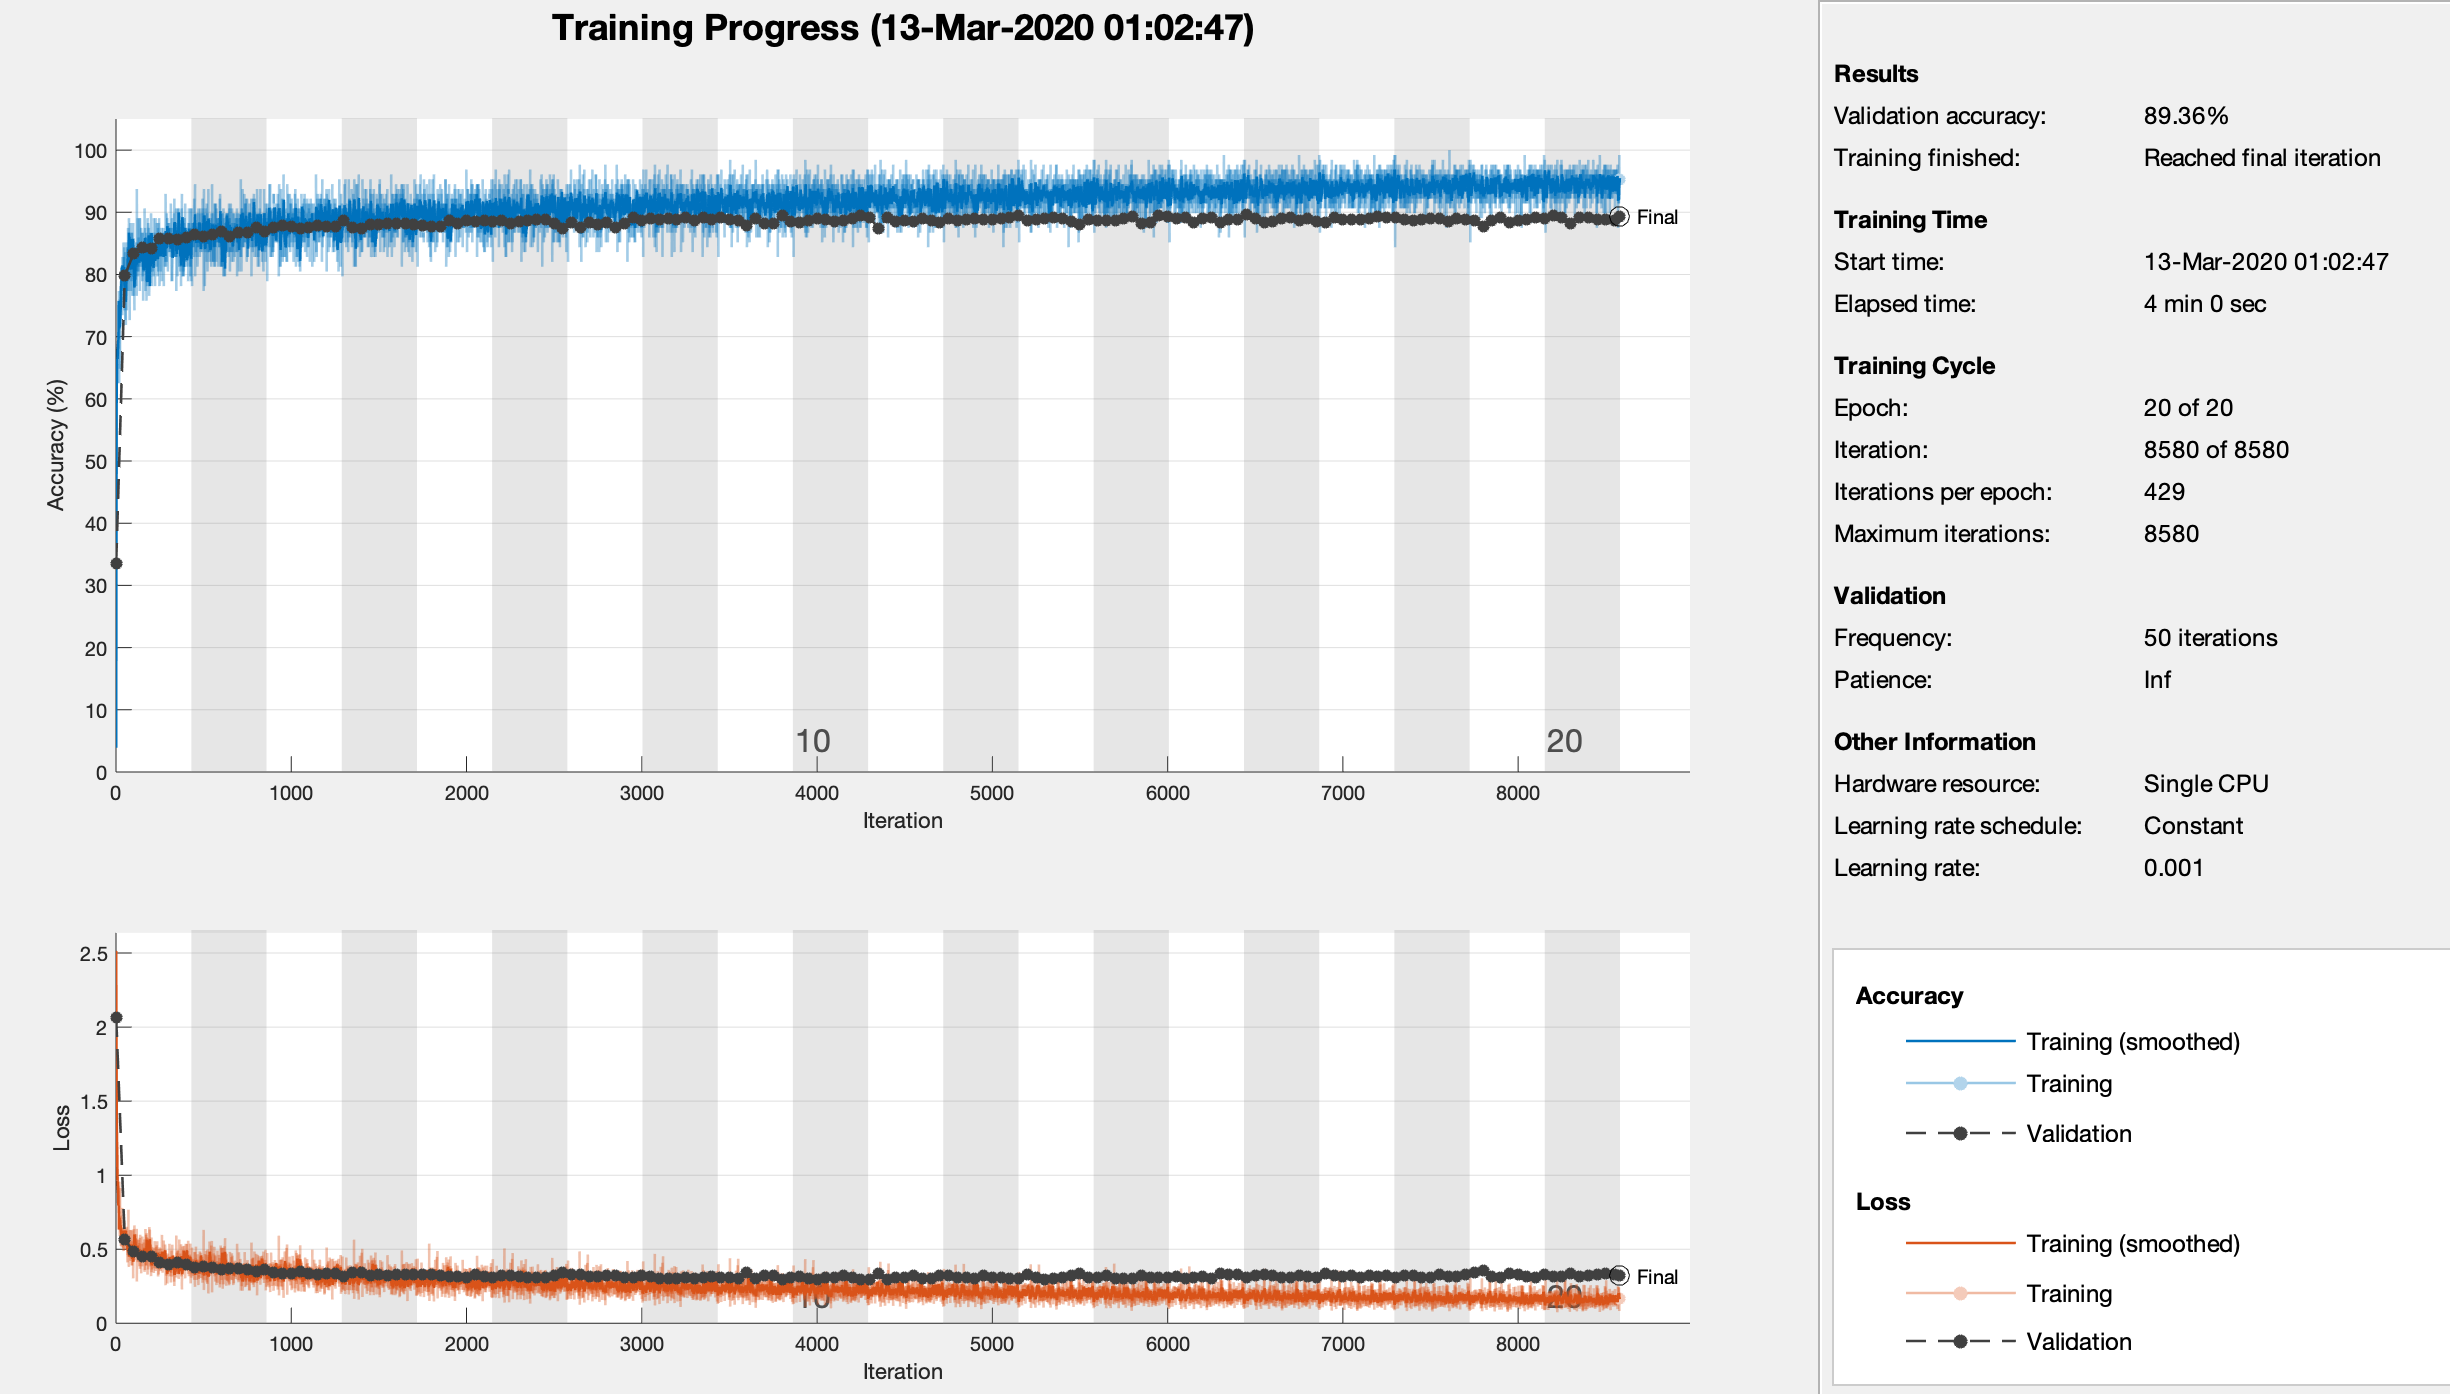
\includegraphics[width=1\linewidth]{1-a.png}  
  \caption{Trace Plot}
  \label{fig:sub-first}
\end{subfigure}
\begin{subfigure}{.5\textwidth}
  \centering
  % include second image
  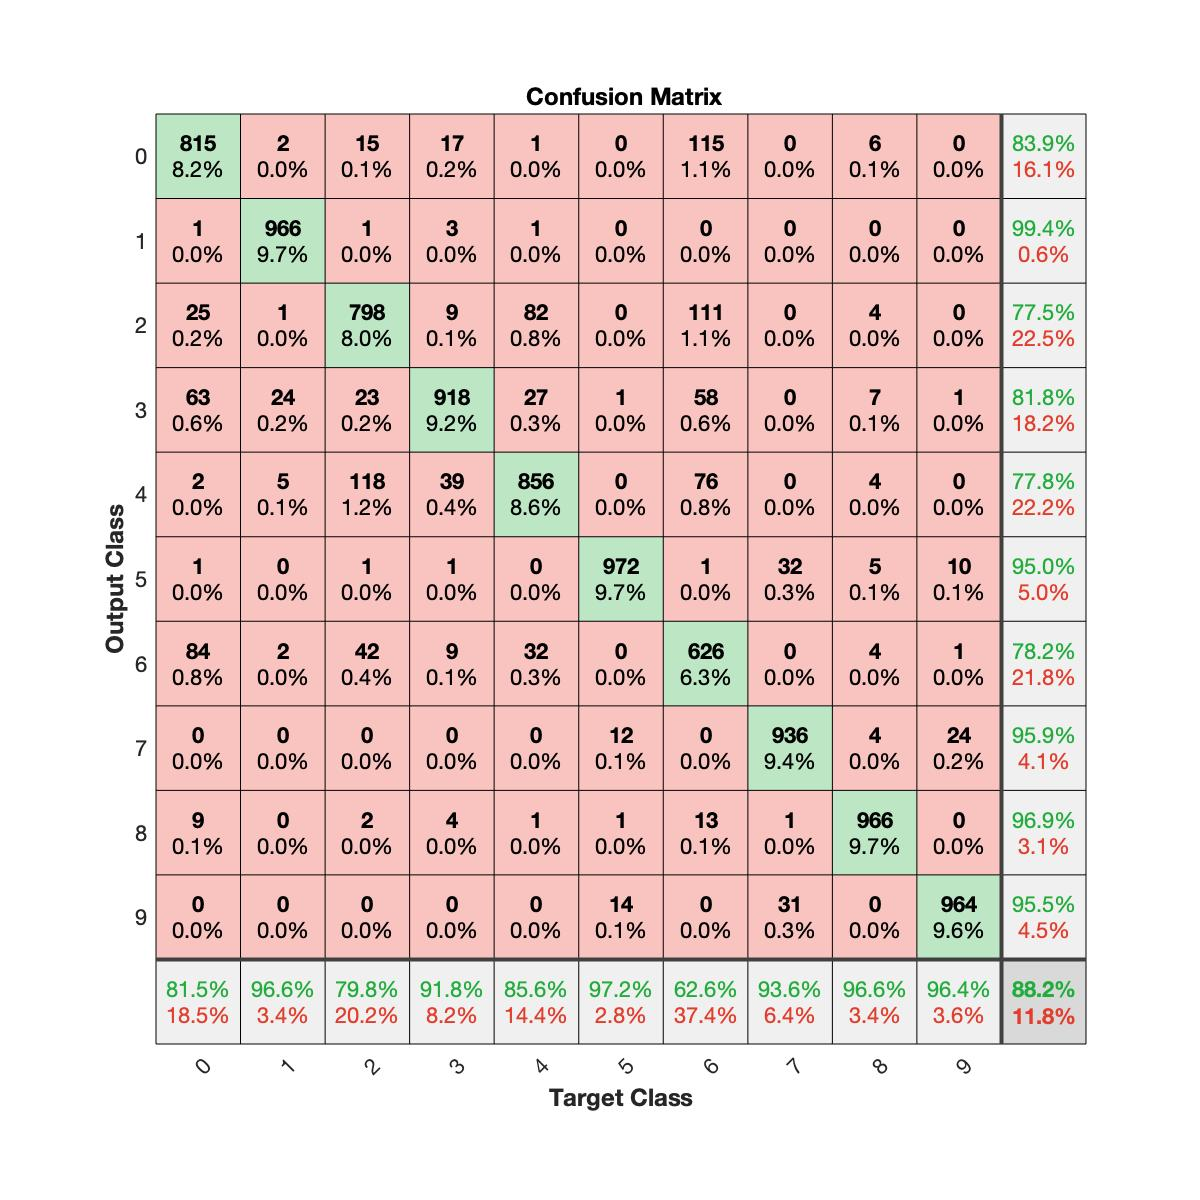
\includegraphics[width=1\linewidth]{1-b.jpg}  
  \caption{Confusion Matrix}
  \label{fig:sub-second}
\end{subfigure}
\label{fig:fig}
\caption{ }
\end{figure}
From the trace plot (Figure 1a), we can see that there's not serious overfitting problem, because the validation line overlaps with the training line for the first 10 epoch but deviate a little later. From the confusion matrix(Figure 1b), we can see that the full-connected neural networks often misclassified 0 as 6, 2 as 4 and 2 as 6, which makes sense because 0 (Top), 6(Shirt) looks similar execpt for the length of the sleeve; 2(Pullover) and 6(Top) look very similar except for the texture of the clothe; 2(Pullover) and 4(coat) also look similar except for the existence of a hat. 

\subsection*{Part II}
As I mentioned before, I decided my final convolutional neural network model structureof the third experiment I did. At the 5th epoch, the validation accuracyis $91.1\%$ and the training accuracy is $94\%$. For the testing data, the prediction accuracy is $90.7\%$ given by the following confusion matrix. 

\begin{figure}[ht]
\begin{subfigure}{.5\textwidth}
  \centering
  % include first image
  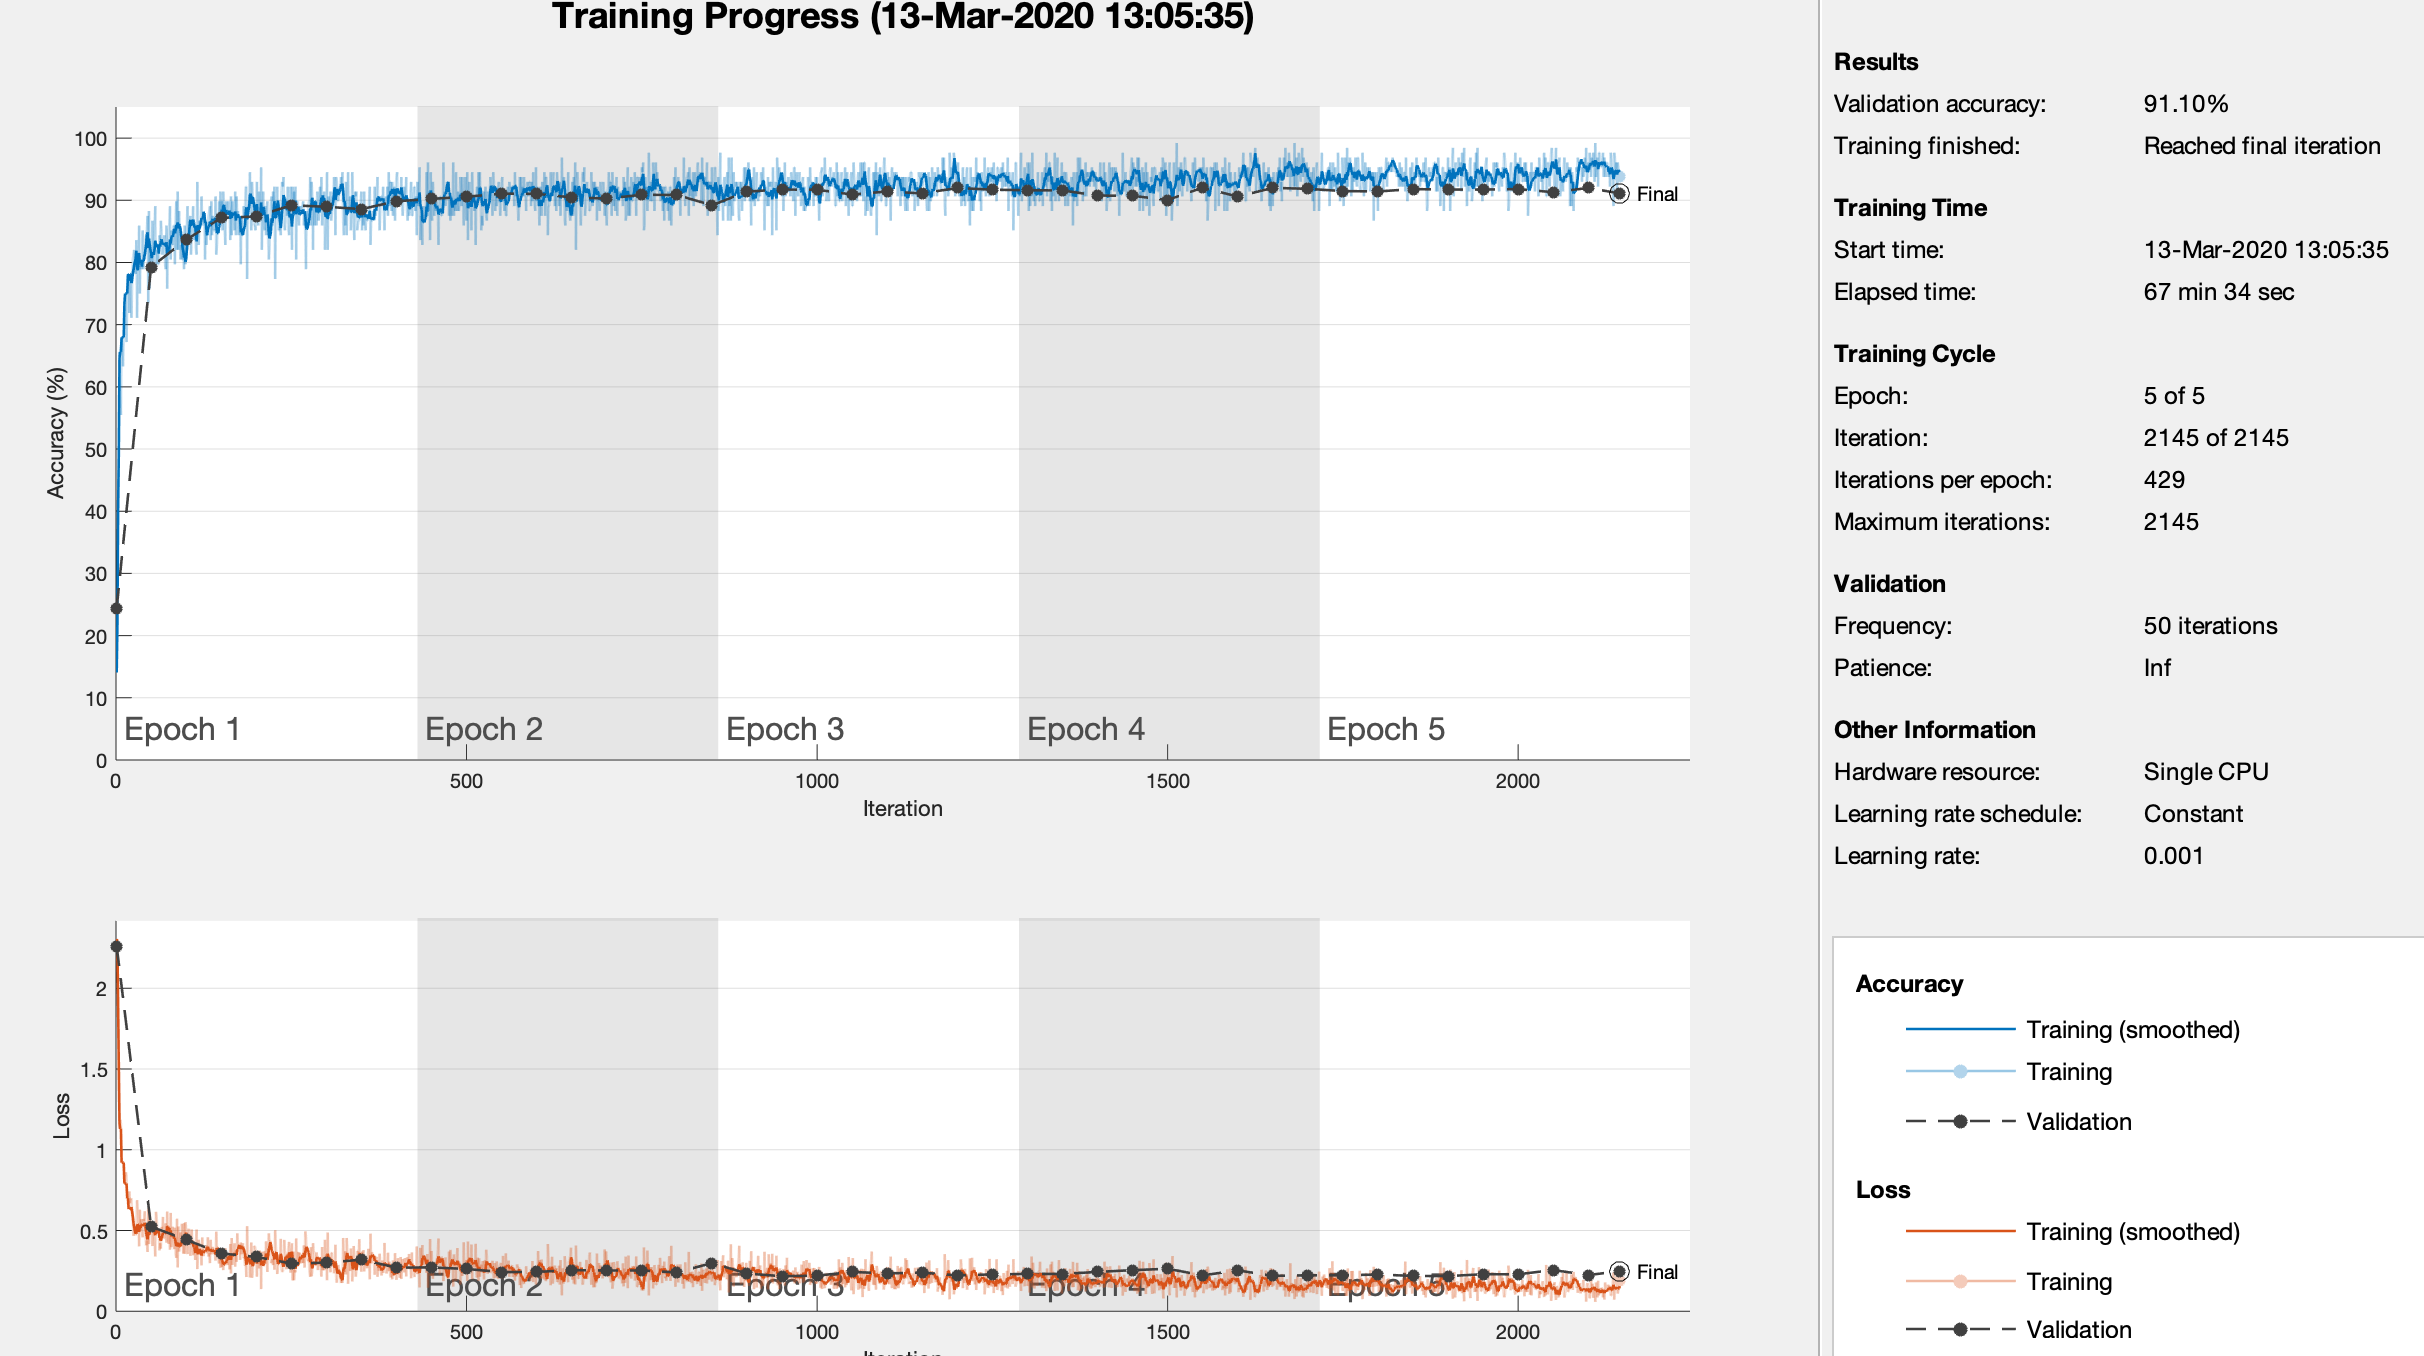
\includegraphics[width=1\linewidth]{2-a.png}  
  \caption{Trace Plot}
  \label{fig:sub-first}
\end{subfigure}
\begin{subfigure}{.5\textwidth}
  \centering
  % include second image
  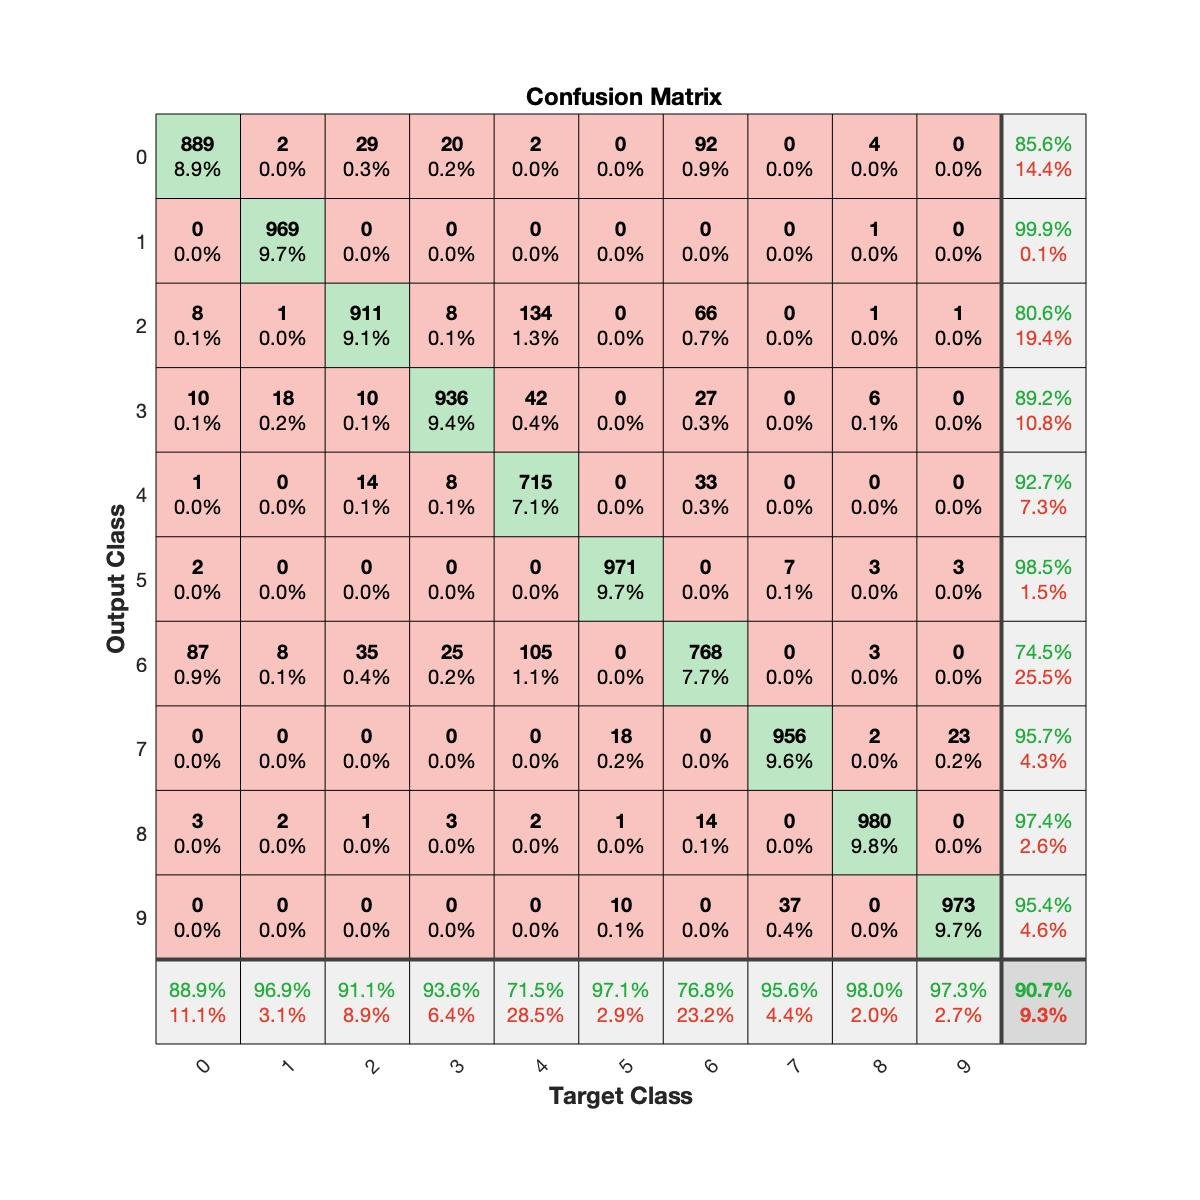
\includegraphics[width=1\linewidth]{2-b.jpg}  
  \caption{Confusion Matrix}
  \label{fig:sub-second}
\end{subfigure}
\label{fig:fig}
\caption{ }
\end{figure}
From the trace plot (Figure 2a), we can see that there's not serious overfitting problem, because the validation line overlaps with the training line.  From the confusion matrix(Figure 2b), we can see that the convolutional neural networks often misclassified 0 as 6, 2 as 4 and 2 as 6, which makes sense because 0 (Top), 6(Shirt) looks similar execpt for the length of the sleeve; 2(Pullover) and 6(Top) look very similar except for the texture of the clothe; 2(Pullover) and 4(coat) also look similar except for the existence of a hat. 

\section*{V. Summary and Conclusions}
For this project, we trained a fully-connected neural network for part I and a convolutional neural network model for part II within a dataset of images of 10 different classes of fashion items. We can see that the convolutional neural network structure is more complex than the fully connected neural networks and works better with a better accuracy. From both model, we can see that it's easy to misclassified 0 as 6, 2 as 4 and 2 as 6, which makes sense because 0 (Top), 6(Shirt) looks similar execpt for the length of the sleeve; 2(Pullover) and 6(Top) look very similar except for the texture of the clothe; 2(Pullover) and 4(coat) also look similar except for the existence of a hat. 

\section*{Appendix A. MATLAB functions used and brief implementation explanation}
im2double: $Xtrain = im2double(X)$ converts the image X to double precision.
\\
\\reshape: $Xtrain = reshape(X,[60000\:28\:28\:1])$ reshapes X into a 6000-28-by-28-by-1array. 
\\
\\permute: $Xtrain = permute(X,[2\:3\:4\:1])$ rearranges the dimensions of X so that they are in the order specified by the vector order.
\\
\\options = trainingOptions(x) returns training options for the optimizer specified by x. 
\\
\\plotconfusion(ytest,ypred)  plots a confusion matrix for the true labels ytest and predicted labels ypred. Specify the labels as categorical vectors, or in one-of-N (one-hot) form.
\newpage
\section*{Appendix B. MATLAB codes}
\begin{verbatim}
clear; close all; clc;
%% part 1
load("fashion_mnist.mat");

X_train = im2double(X_train);
X_test = im2double(X_test);
X_train = reshape(X_train,[60000 28 28 1]);
X_train = permute(X_train,[2 3 4 1]);
X_test = reshape(X_test,[10000 28 28 1]);
X_test = permute(X_test,[2 3 4 1]);
X_valid = X_train(:,:,:,1:5000);
X_train = X_train(:,:,:,5001:end);

y_valid = categorical(y_train(1:5000))';
y_train = categorical(y_train(5001:end))';
y_test = categorical(y_test)';


layers = [imageInputLayer([28 28 1])
        fullyConnectedLayer(250)
        reluLayer
        fullyConnectedLayer(10)
        softmaxLayer
        classificationLayer];

options = trainingOptions('adam', ...
    'MaxEpochs',20,...
    'InitialLearnRate',1e-3, ...
    'L2Regularization',1e-4, ...
    'ValidationData',{X_valid,y_valid}, ...
    'Verbose',false, ...
    'Plots','training-progress');

net = trainNetwork(X_train,y_train,layers,options);
%%
figure(1)
plotperf(net)

%% figure(3)
y_pred = classify(net,X_test);
plotconfusion(y_test,y_pred)

%% part 2
load("fashion_mnist.mat");

X_train = im2double(X_train);
X_test = im2double(X_test);

X_train = reshape(X_train,[60000 28 28 1]);
X_train = permute(X_train,[2 3 4 1]);

X_test = reshape(X_test,[10000 28 28 1]);
X_test = permute(X_test,[2 3 4 1]);

X_valid = X_train(:,:,:,1:5000);
X_train = X_train(:,:,:,5001:end);

y_valid = categorical(y_train(1:5000))';
y_train = categorical(y_train(5001:end))';
y_test = categorical(y_test)';


layers = [
    imageInputLayer([28 28 1],"Name","imageinput")
    convolution2dLayer([3 3],32,"Name","conv_1","Padding","same")
    reluLayer("Name","relu_1")
    maxPooling2dLayer([2 2],"Name","maxpool_1")
    convolution2dLayer([3 3],64,"Name","conv_2")
    reluLayer("Name","relu_2")
    maxPooling2dLayer([2 2],"Name","maxpool_2")
    convolution2dLayer([3 3],128,"Name","conv_3")
    reluLayer("Name","relu_3")
    fullyConnectedLayer(256,"Name","fc_1")
    reluLayer("Name","relu_4")
    fullyConnectedLayer(10,"Name","fc_2")
    softmaxLayer("Name","softmax")
    classificationLayer("Name","classoutput")];

options = trainingOptions('adam', ...
    'MaxEpochs',5,...
    'InitialLearnRate',1e-3, ...
    'L2Regularization',1e-4, ...
    'ValidationData',{X_valid,y_valid}, ...
    'Verbose',false, ...
    'Plots','training-progress');

net = trainNetwork(X_train,y_train,layers,options);
%%
figure(1)
y_pred = classify(net,X_train);
plotconfusion(y_train,y_pred)

%% Test classifier
figure(2)
y_pred = classify(net,X_test);
plotconfusion(y_test,y_pred)
\end{verbatim}



\end{document}